\begin{figure}[h!]
	\centering
	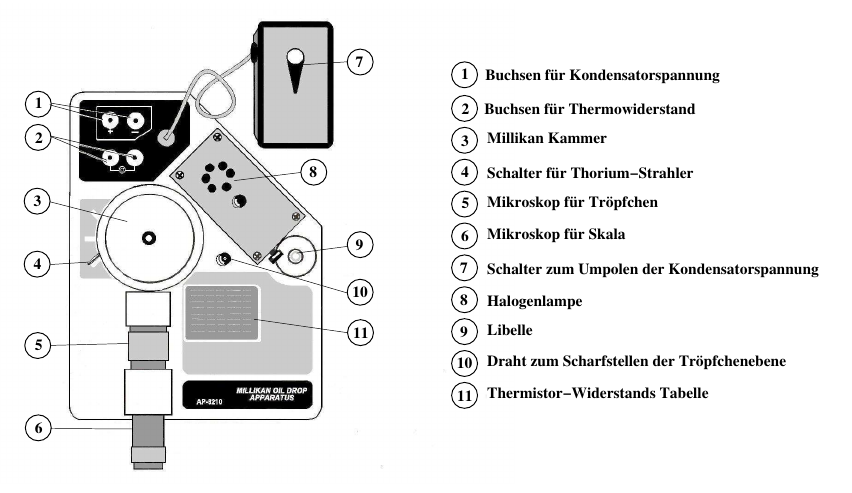
\includegraphics[width=\textwidth]{Versuchsaufbau.png}
	\caption{Versuchsaufbau Millikan-Öltröpfchenversuch \cite{V503}}
	\label{fig:versuchsaufbau}
\end{figure}


Das zentrale Element des Millikan-Versuchs (siehe Abbildung \ref{fig:versuchsaufbau}) ist ein waagerechter Plattenkondensator in der sogenannten Millikan Kammer {\large\textcircled{\normalsize \texttt{3}}}. Der Plattenabstand beträgt \SI{7.6259+-0.0051}{\milli\meter}. In die Millikan Kammer werden mit Hilfe eines Zerstäubers kleine Öltröpfchen gegeben, die angestrahlt {\large\textcircled{\normalsize \texttt{8}}} und durch ein Mikroskop {\large\textcircled{\normalsize \texttt{5}}} am Bildschirm beobachtet werden. Eine Längenskala {\large\textcircled{\normalsize \texttt{6}}} erlaubt es, die von den Tropfen zurückgelegte Strecke genau zu bestimmen. Zusätzlich wird die Zeit mit einer Stoppuhr gemessen, sodass die Geschwindigkeit der Tropfen berechnet werden kann. Für jeden ausgewählten Tropfen wird eine Geschwindigkeit ohne angelegte Spannung und jeweils mehrere\todo[color = yellow]{Hier habe ich 'drei' in 'mehrere' verändert, da es immer unterschiedlich viele waren.} Fall-/Steigeschwindigkeiten pro negativer/positiver Kondensatorspannung gemessen. Die Kondensatorspannung kann variiert werden {\large\textcircled{\normalsize \texttt{1}}}, sollte jedoch \SI{500}{\volt} nicht überschreiten. Falls die Tröpfchen zu wenige Ladungen tragen, können sie kurzzeitig mit einem radioaktiven Präparat {\large\textcircled{\normalsize \texttt{4}}} bestrahlt werden. \\
Aus den Messungen kann die Ladung und der Radius der Öltröpfchen berechnet werden und die Elementarladung als größte gemeinsame Vielfache der gemessenen Ladungen identifiziert werden. \\
Des weiteren muss die Temperatur in der Kammer überprüft werden {\large\textcircled{\normalsize \texttt{2}}}, um sicherzustellen, dass die Viskosität sich während der Messung nicht zu sehr ändert.
{\large\textcircled{\normalsize \texttt{1}}}